% Diagram: 3-step process with a decision diamond.
% Coordinates: (x, y)
%   start at (0, 3)    -- top, entry
%   decide at (0, 1.5) -- middle, branch point
%   yes at (-3, 0)     -- lower left, yes path
%   no  at (3, 0)      -- lower right, no path
%
% Embeds P1 (explicit node dims), P2 (this comment), P4 (directional labels).
\documentclass[border=4pt]{standalone}
\usepackage{tikz}
\usetikzlibrary{positioning, arrows.meta, shapes.geometric, shapes.misc}
\begin{document}
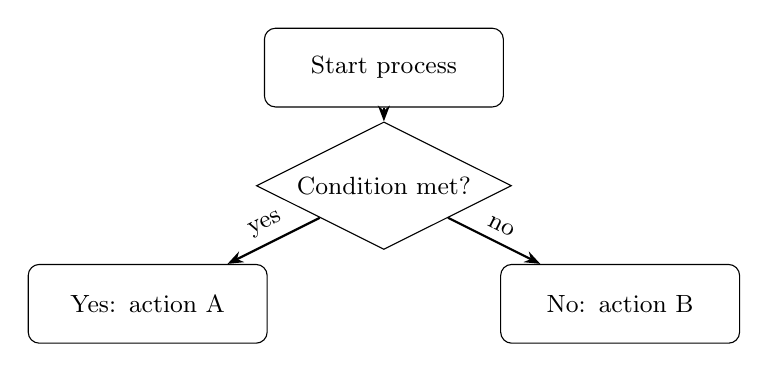
\begin{tikzpicture}[
    node distance=1cm,
    every node/.style={font=\small},
    box/.style={draw, rounded corners,
                minimum width=3cm, minimum height=1cm,
                text width=2.8cm, align=center},
    decision/.style={draw, diamond, aspect=2,
                     minimum width=3cm, minimum height=1.2cm,
                     text width=2.8cm, align=center, inner sep=0pt},
    arrow/.style={-{Stealth[length=2mm]}, thick}
  ]
  \node[box]      (start)  at (0, 3)    {Start process};
  \node[decision] (decide) at (0, 1.5)  {Condition met?};
  \node[box]      (yes)    at (-3, 0)   {Yes: action A};
  \node[box]      (no)     at (3, 0)    {No: action B};

  \draw[arrow] (start)  -- (decide);
  \draw[arrow] (decide) -- (yes) node[midway, above, sloped] {yes};
  \draw[arrow] (decide) -- (no)  node[midway, above, sloped] {no};
\end{tikzpicture}
\end{document}
